\section{Networking}



If the 3D renderer was breathtaking, it was the networking capability and its famous deathmatchs which really took \doom{} to a new level. The ability to connect two PCs and interact with human players was something completely new back then. Early one during development it was apparent this aspect of the game was going to be amazing.\\
\par
\fq{I still remember the day that multiplayer started just barely working in Doom. I had two DOS boxes set up in my office in addition to my NeXT workstation to test multiplayer. The IPX networking was forwarding user input between the systems, but there was no error recovery, so it was very fragile. Still, I could spawn two marines in a test level, and they could look at each other.\\
\par
I was strafing back and forth on one system and looking over my shoulder at the other computer, watching the marine sprite slide side to side in front of the other player's pistol. I let it coast down, centered on the screen, and turned to the other computer. "Bang!" "Urgh!" Twitch. Shuffle. Big smile. :-) "Bang!" "Bang!" "Bang!" "Bang!" There was a consistency failure before the first frag was truly logged, but it was blindingly obvious that this was going to be awesome.}{John Carmack, kotaku.com "Memories Of Doom"}\\
\par



\subsection{Architecture}
Most modern FPS games are designed around a concept of Client/Server where there are several clients and one source of truth, the server. Clients can join a game anytime, they send their commands to the server, receive world updates, and perform prediction to minimize communications latency.\\
\par
\begin{wrapfigure}[9]{r}{0.3\textwidth}
\centering
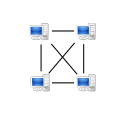
\includegraphics[width=.3\textwidth]{drawings/p2psvg.pdf}
\end{wrapfigure}
There are no central server in \doom. All peers runs their own game logic and remain in sync by performing no predictions and only running a game tic when all other peers actions are known.\\
\par
 This means all peers must advertise their command to all other peers, resulting in significant communication overhead. 
All peers must be present when a game starts. A player an leave (and it will just stay still in the game without performing any action) but new players cannot join.
\pagebreak
 % Each node must send the command generated locally to all other nodes. This means that a machine can simulate the next tic only when ALL nodes involved in the game have send their commands. As a result, the slowest machine dictates the framerate of every players involved. This also meant that all nodes had to run the exact same state machine and run the same version of \doom.\\
% \par





On NeXT, the implementation used a simple UDP system with Berkley sockets\footnote{The Internet Assigned Numbers Authority (IANA) publishes a list, The Service Name and Transport Protocol Port Number Registry where UDP port 666 is reserved for \doom!}. On the PC side, things were more complicated. Until v1.1 the game engine shipped with built-in support for LAN over IPX. To minimize communications, Dave Taylor suggested to use ipx packet node number \cw{FF-FF-FF-FF-FF-FF} in order to broadcast updates and reduce the amount of communications. However things did not go as smoothly as expected.\\
\par
\fq{Doom used IPX broadcast packets to communicate between the players. This seemed like a good efficiency to me a four player game just involved four broadcast packets each frame. My knowledge of networking was limited to the couple of books I had read, and my naive understanding was that big networks were broken up into little segments connected by routers, and broadcast packets were contained to the little segments. I figured I would eventually extend things to allow playing across routers, but I could ignore the issue for the time being.\\
\par
What I didn't realize was that there were some entire campuses that were built up out of bridged IPX networks, and a broadcast packet could be forwarded across many bridges until it had been seen by every single computer on the campus. At those sites, every person playing LAN Doom had an impact on every computer on the network, as each broadcast packet had to be examined to see if the local computer wanted it. A few dozen Doom players could cripple a network with a few thousand endpoints.\\
\par
The day after release, I was awoken by a phone call. I blearily answered it and got chewed out by a network administrator who had found my phone number just to yell at me for my game breaking his entire network. I quickly changed the network protocol to only use broadcast packets for game discovery, and send all-to-all directed packets for gameplay (resulting in 3x the total number of packets for a four player game), but a lot of admins still had to add Doom-specific rules to their bridges (as well as stern warnings that nobody should play the game) to deal with the problems of the original release.}{John Carmack, kotaku.com "Memories Of Doom"}\\ 
\par
With the proliferation of networking medium, the embedded IPX support started to show its limit.\\
\par
 Instead of baking in the engine support for more types of network, the IPX network system was removed and networking was refactored around the notion of network drivers.
\pagebreak



% \par
% \begin{verbatim}

%  IPX addressing: 12 bytes structured as follow:

%    Network         Node        Socket
% |-----------|-----------------|-----|
%  XX XX XX XX XX XX XX XX XX XX XX XX 

% \end{verbatim}


\subsection{PC Network drivers}
In this model, the game engine deals with a datastructure named \cw{doomcom\_t} (detailed on page \pageref{doomcom_t.c}) located in shared memory. Receiving or emitting packet is done via interrupts. How this all worked together is a magnificent hack like only an unprotected OS allowed.\\
\par
The driver must start first and install itself as a tiny TSR interrupt handler in RAM. The driver then start \cw{DOOM.EXE} with a special parameter \cw{-net X} where X is the address of the TSR \cw{doomcom\_t} variable. The engine literaly did a \cw{(doomcom\_t*)(atoi(param))} to access the structure fields.\\
\par

\fakedosoutput{doomnet.c}
\par
 At this point, the engine has everything it needs to communicate in a generic way. It writes or read from \cw{doomcom\_t} and triggers read/write via the interrupt number (also provided in \cw{doomcom\_t}).\\
\par
\drawing{net_drivers}{}
\par
\circled{1} \cw{IPXSERVER.EXE} starts, becomes a TSR and register itself in the software Interrupt Vector Table, \circled{2} \cw{IPXSERVER.EXE} start \cw{DOOM.EXE} and pass the address of its \cw{doomcom\_t} variable, \circled{3} \cw{DOOM.EXE} write/read in the \cw{doomcom\_t} \cw{payload} field and trigger transfer via interrupt number found in \cw{intnum} field, \circled{4} the \doom{} network driver communicate with the network card driver, \circled{5} the network card driver communicate with the actual network card.\\
\par
Two drivers shipped with the game, \cw{IPXSETUP.EXE} which allowed up to four nodes over IPX, and \cw{SERSETUP.EXE} which allowed two players over serial cable or modem.






\subsection{Implementation}
To perform network I/O, the core only deals with three elements provided by the Network system.\\
\par
 \begin{figure}[H]
\centering  
\begin{tabularx}{\textwidth}{ L{0.6}  L{1.4}}
  \toprule
  \textbf{Element} &  \textbf{Usage}\\

  \toprule 
   I\_InitNetwork & Initialize the network system.\\
   \cw{doomcom\_t doomcom} & Shared structure containing both in and out data.\\
   I\_NetCmd & Signal network to send/receive data based on doomcom.\\
   \toprule
\end{tabularx}
\caption{\doom network system interface}
\end{figure}



On PC, in the case of a multi-player session, the network initialization simply retrieve the address of the TSR.\\
\par
\ccode{I_InitNetwork.c}\\
\par
With access to the \cw{doomcom} variable, come access to the field \cw{intnum} which is the software interrupt the network TSR registered itself with. Raising this interrupt will halt \doom{} to let the network driver copy network data in or out of \cw{doomcom}.\\



\ccode{doomcom_t.c} \label{doomcom_t.c} \\
\par
The fields are self explanatory but notice \cw{command} which indicate the driver if data should be read or sent. Notice field \cw{id} which allows \doom{} to verify the address alleged to be a TSR was correct. Notice the \cw{ticcmd\_t} payload which was already studied in the input system on page \pageref{cmd_t_type}.



At a high level, the Core uses a central method called \cw{Net\_Update} to do all I/O. Notice how it is called in a loop as long as all the cmd tic for all peers have not been received, allowing only menus to keep on working. Except for running menus, nothing else will run.\\
\par
\ccode{net_loop_wait.c}\\
\par
The impossibility for the engine to extrapolate and carry on with gameplay was an issue since all machines ended up running a the lowest common framerate. To mitigate this issue, the engine perform an exotic "thread multiplexing" where \cw{NetUpdate} is found called several times during a frame. It is typically called no less than eight times.\\
\par
\ccode{R_RenderPlayerView_withupdates.c}



There is not expectation the medium will guarantee packet delivery so the engine features a negative acknowledgment where packet sequential number is tracked on a per peer (a.k.a node) basis. If a packet is received but its serial number indicates a previous packet was lost, the node requests the missing commands to be sent again. This meant each node cannot discard commands once they were sent on the wire.\\
\par
This resent mechanism was a last resort to be avoided at all cost. To this effect, packets feature not only the current command but also the last command (field \cw{extratics} is marked as true).\\





\subsection{DeathManager}
Given the complexity of the commandline parameters to setup a network game, several tools were provided. Originally players could use \cw{SETUP.EXE}. Later version showed the introduction of \cw{DM.EXE} (DeathManager) which was easier to use.\\
\par
\fullimage{DeathManagerv1-2.png}\\
\trivia{DeathManager appears to have been written in Turbo C. Unlike the other utilities, the source code to DeathManager has never been released.}\\
\par











\trivia{The "official" (as stated in the IPXSETUP source code) IPX socket number for \doom{} is 869C hex (34460 decimal). This was apparently registered with Novell, as it appears in the list of well-known IPX sockets published by Novell.}

\fullimage{coop.png}\\
\par
Co-op play was fun (above) but so were incredibly bloody deathmatchs (below).\\
\par
\fullimage{deathmatch.png}


